The next part to be measured is the ADC. This is an important step, because the ADC is actually 
our eyes on the system regarding the position of the wings (as well some other indicators about
different power rails on the system).

It's important for us to be confident in it's measure, so we did some measurement on it to identify 
it's limitations and workarounds.

\paragraph{}
We used this schematic for this measurement session :
\begin{figure}[!hbt]
    \centering

    \begin{circuitikz}
        % ---------------------------------------------------------------------------
        % Draw components
        % ---------------------------------------------------------------------------
        % ADC + MCU + MUX
        \draw (8,3) node[msport, circuitikz/RF/scale=2](ADC){ADC};
        \draw (ADC.right) ++(0.5,0) node[twoportshape, anchor=left, t=Core](uC){};
        \draw (ADC.left) ++(-1.5, 0) node[muxdemux] (Mux) {Mux};

        % Vsources
        \draw (0,0) node[ground] () {}     to[vsource]     ++(0,1.5);
        \draw (1.5,0) node[ground] () {}     to[vsource]     ++(0,1.5);

        % ---------------------------------------------------------------------------
        %  Boxes
        % ---------------------------------------------------------------------------
        \node [rectangle, draw, dashed, fit=(ADC) (uC) (Mux)](MCU) {};
        \node [below, align=center] at (MCU.south) {MCU (nRF5340)} ;

        % ---------------------------------------------------------------------------
        % Draw wires
        % ---------------------------------------------------------------------------
        \draw (ADC.right) -- (uC.left);
        \draw (Mux.rpin 1) -- (ADC.left);

        \draw (0, 1.5) -- (0, 1.5 |- Mux.blpin 1) -- (Mux.blpin 1);
        \draw (1.5, 1.5) -- (1.5, 1.5 |- Mux.blpin 2) -- (Mux.blpin 2);

        \draw (Mux.blpin 3) to[short, -o]    ++(-1,0);
        \draw (Mux.blpin 4) to[short, -o]    ++(-1,0);
        \draw (Mux.blpin 5) to[short, -o]    ++(-1,0);
        \draw (Mux.blpin 6) to[short, -o]    ++(-1,0);
        \draw (Mux.blpin 7) to[short, -o]    ++(-1,0);
        \draw (Mux.blpin 8) to[short, -o]    ++(-1,0);
        
    \end{circuitikz}
    
    \caption{Schematic used for testing response of the ADC core of the MCU}
    \label{fig:ADC_test}
\end{figure}

We sent different voltages waveforms on the ADC core, including :

\begin{itemize}
    \item Precise DC voltages
    \item Voltages ramps
\end{itemize}

Now, let's dig into the different measures we did :

\FloatBarrier
\subsection{Time deviation}
The first parameter we did measure is the time deviation. Does the ADC drift with the time / heat ?
To measure that, we sent precise voltages to the ADC inputs, voltages that we know they won't drift.

And then, we recorded over a long time (~ 20 mn) the values, and plotted them on a graphe.

\begin{figure}[!hbt]
    \centering
    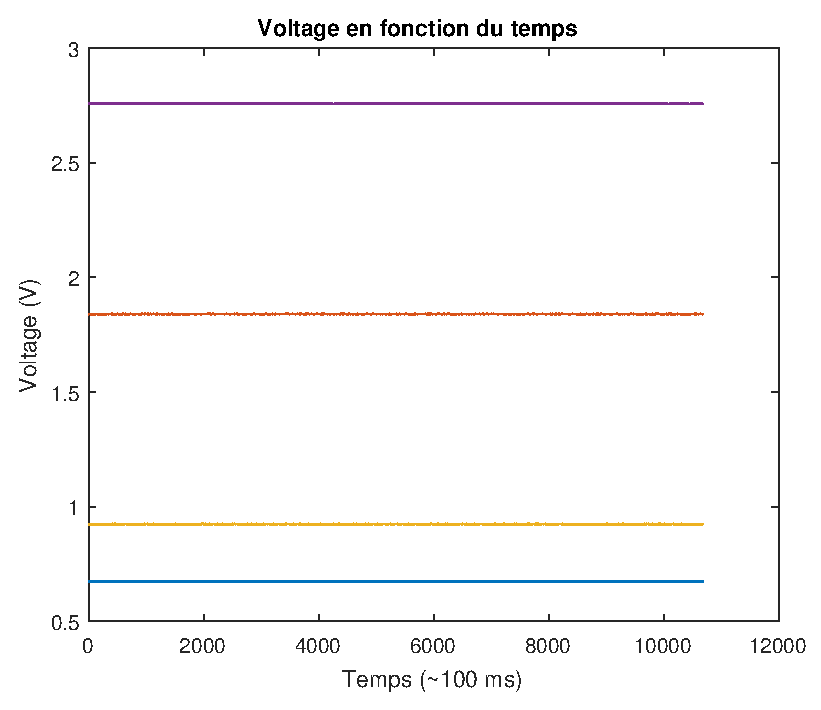
\includegraphics[width=\SchematicWidth]{\Images/ADC/time-deviation.eps}
    \caption{ADC drift over time}
\end{figure}
\FloatBarrier

Here, we can clearly see that the ADC does not seems to deviate at all, so that's a good point ! We 
know that it's transfer function can be expressed as $N = f(V)$ and does not depend on the time.

\FloatBarrier
\subsection{Non linearity}
The second parameter to be measured is the linearity of the ADC. We need to know if the response of 
the ADC is linear. This is important, becase we'll be using the ADC as position sensor.

To measure that, the voltage sources were configured as ramp input, and we recorded output values over
a long time (~45 mn) to cover a large number of periods of the input ramp, which was slow to let time
to the ADC to convert.

\begin{figure}[!hbt]
    \centering
    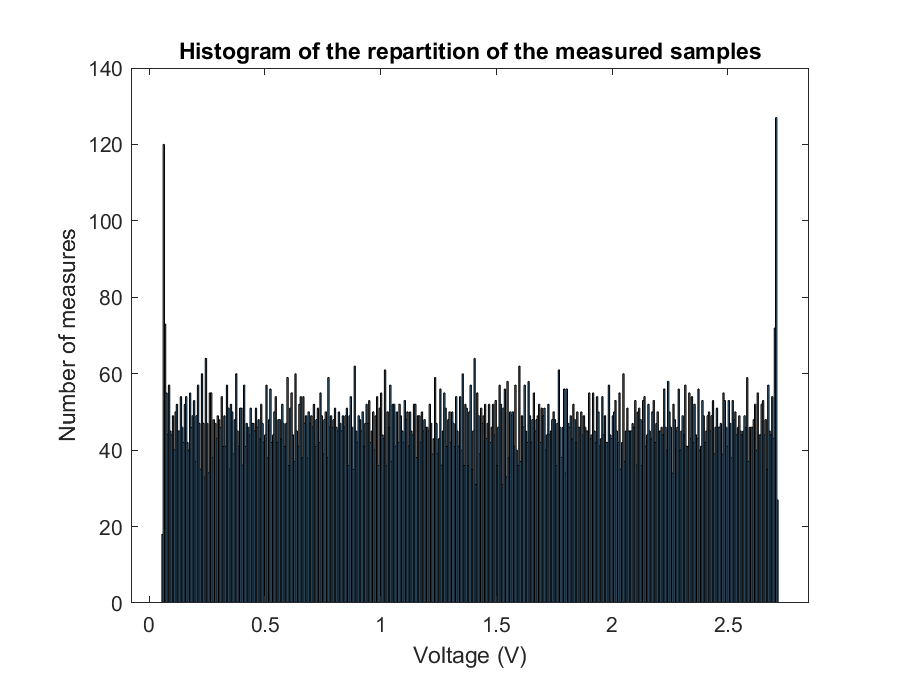
\includegraphics[width=\SchematicWidth]{\Images/ADC/ADC-DNL.eps}
    \caption{ADC drift over time}
\end{figure}
\FloatBarrier

\paragraph{}
The result here is typical from integrated ADC. Theses graphics represent the number of times there was this
voltage at it's inputs during the test. 
A perfect ADC shall return the exact same number for all voltages (Since a ramp is by definition linear).

\paragraph{}
Here, we're not observing that. In the middle of the voltage range, the codes are evenly distributed, which
mean that the ADC is quite linear here. But on the extreme, we can clearly see two spikes, which means the ADC 
isn't able to differentiate voltages here (they will, in any case produce the same code).

This should not cause any issues here, because our return signal is included between $600 \si{\milli\volt}$ 
and $2.4 \si{\volt}$, which by chance is in the correct range. Otherwise, it would require some amplification
or offset to get the needed precision.


\FloatBarrier
\subsection{Gain error}
The last point that is required here is the gain error. Since the internal components of the ADC include
an amplifier and some analog front-end, we need to make sure that they not add some unwanted errors.

To measure that, we send precises voltages to the inputs, and log the output voltage.
Then, with a simple division we can estimate the gain error.

This gave us theses plots :
\begin{figure}
    \centering
    \subfloat[\centering Raw measures]{{\includegraphics[width=\SmallSchematicWidth]{\Images/ADC/gain-error.eps} }}%
    \qquad
    \subfloat[\centering Corrected measures]{{\includegraphics[width=\SmallSchematicWidth]{\Images/ADC/gain-compensated.eps} }}%
    \caption{Uncorrected and corrected gain errors}%
\end{figure}
\FloatBarrier



